\chapter[Suất điện động tự cảm - Năng lượng từ trường của ống dây tự cảm]{Suất điện động tự cảm \\ Năng lượng từ trường của ống dây tự cảm}
\section{Lý thuyết trọng tâm}
\subsection{Suất điện động tự cảm}
Khi có hiện tượng tự cảm xảy ra trong một mạch điện thì suất điện động cảm ứng xuất hiện trong mạch được gọi là suất điện động tự cảm.

Giá trị của nó được tính theo công thức:

\begin{equation}
e_\text{tc}=-\dfrac{\Delta \Phi}{\Delta t},
\end{equation}
trong đó, $\Phi$ là từ thông riêng được cho bởi: $\Phi=Li$.

Vì độ tự cảm $L$ không đổi, nên $\Delta \Phi=L\Delta i$.

Vậy, suất điện động tự cảm có công thức:
\begin{equation}
e_\text{tc}=-L\dfrac{ \Delta i}{\Delta t},
\end{equation}
\begin{itemize}
	\item $\Delta i$ là độ biến thiên cường độ dòng điện,
	\item $\Delta t$ là khoảng thời gian, 
	\item $e_\text{tc}$ là suất điện động tự cảm. 
\end{itemize}

Về độ lớn:

\begin{equation}
\left| e_\text{tc}\right| =\left| -L\dfrac{ \Delta i}{\Delta t}\right| ,
\end{equation}

Suất điện động tự cảm có độ lớn tỉ lệ với tốc độ biến thiên của cường độ dòng  điện trong mạch.

\subsection{Năng lượng từ trường của ống dây tự cảm}

\begin{equation}
W=\dfrac{1}{2}Li^2,
\end{equation}
trong đó,
\begin{itemize}
	\item $L$ là độ tự cảm,
	\item $i$ là cường độ dòng điện trong ống dây, 
	\item $W$ là năng lượng từ trường của ống dây tự cảm. 
\end{itemize}
\section{Bài tập}
\begin{dang}{Suất điện động tự cảm}
\end{dang}

\textbf{Phương pháp giải}

Độ tự cảm $L$ được tính theo công thức:
\begin{equation}
L=4\pi \cdot 10^{-7}\cdot \dfrac{N^2}{l}\cdot S,
\end{equation}
hay 
\begin{equation}
L=4\pi \cdot 10^{-7}\cdot n^2 \cdot V,
\end{equation}

Công thức tính suất điện động cảm ứng:
\begin{equation}
e_\text{tc}=-L\dfrac{ \Delta i}{\Delta t},
\end{equation}

Về độ lớn:

\begin{equation}
\left| e_\text{tc}\right| =\left| -L\dfrac{ \Delta i}{\Delta t}\right|,
\end{equation}
\vspace{1em}
{\viduii{2}{	
Một ống dây dài 40 cm, có tất cả 800 vòng dây, diện tích tiết diện ngang của ống dây bằng $10\ \text{cm}^2$. Ống dây được nối với 1 nguồn điện có cường độ tăng từ 0 đến 4 A. Biết độ lớn suất điện động tự cảm của ống dây có độ lớn là $\text{1,2}\ \text{V}$, thời gian mà dòng điện đã biến thiên là
	\begin{mcq}(4)
		\item $\text{6,7}\cdot 10^{-3}\ \text{s}$.
		\item $\text{8}\cdot 10^{-3}\ \text{s}$
		\item $\text{6,7}\ \text{s}$.
		\item  $\text{8}\ \text{s}$.
		
	\end{mcq}}{
\begin{center}
		\textbf{Hướng dẫn giải:}
\end{center}
	
Độ tự cảm của ống dây: $L=4\pi \cdot 10^{-7}\cdot \dfrac{N^2}{l}\cdot S=2\cdot 10^{-3}\ \text{H}$.

Độ lớn suất điện động tự cảm:

$\left| e_\text{tc}\right| =\left| -L\dfrac{ \Delta i}{\Delta t}\right|$

$\Rightarrow \Delta t=L\left|\dfrac{\Delta i}{e_\text{tc}} \right|=\text{6,7}\cdot 10^{-3}\ \text{s}$.
	
\textbf{	Đáp án: A.}
}}

{\viduii{2}{	
Một ống dây dài được quấn với mật độ 2000 vòng/mét. Ống dây có thể tích $500\ \text{cm}^3$. Ống dây được mắc vào một mạch điện. Sau khi đóng công tắc dòng điện trong ống dây biến đổi theo thời gian theo đồ thị. Lúc đóng công tắc ứng với thời điểm $t=0$. 
\begin{center}
	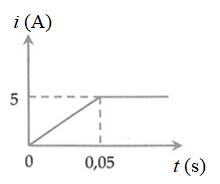
\includegraphics[scale=0.8]{../figs/VN11-PH-31-L-022-2-h71.jpg}
\end{center}
Tính độ lớn của suất điện động tự cảm trong ống:
\begin{enumerate}[label=\alph*)]
	\item Sau khi đóng công tắc tới thời điểm $t=\text{0,05}\ \text{s}$.
	\begin{mcq}(4)
		\item $\text{0,15}\ \text{V}$.
		\item $\text{0,25}\ \text{V}$.
		\item $\text{0,75}\ \text{V}$.
		\item $\text{0,95}\ \text{V}$.
		
	\end{mcq}
		\item Từ thời điểm $t=\text{0,05}\ \text{s}$ trở về sau.
	  
	\begin{mcq}(4)
		\item $0 \ \text{V}$.
		\item  $\text{0,25}\ \text{V}$.
		\item  $\text{0,5}\ \text{V}$.
		\item  $\text{0,75}\ \text{V}$.
		
	\end{mcq}
\end{enumerate}}
{\begin{center}
		\textbf{Hướng dẫn giải:}
\end{center}
	
	Độ tự cảm của ống dây: $L=4\pi \cdot 10^{-7}\cdot n^2 \cdot V=\text{2,51}\cdot 10^{-3}\ \text{H}$.
	
	\begin{enumerate}[label=\alph*)]
		\item Trong khoảng thời gian từ 0 đến $\text{0,05}\ \text{s}$ dòng điện tăng từ $i_1=0\ \text{A}$ đến $i_2=5\ \text{A}$ nên $\Delta i=5\ \text{A}$.
		
		Suất điện động tự cảm trong thời gian này:
		
		$\left| e_\text{tc}\right| =\left| -L\dfrac{ \Delta i}{\Delta t}\right| =\text{0,25}\ \text{V}$.
		
		\textbf{	Đáp án: B.}
			
		\item Từ sau thời điểm $\text{0,05}\ \text{s}$, dòng điện không đổi nên $\Delta i=0\ \text{A}$.
		
		Suy ra $\left| e_\text{tc}\right| =\left| -L\dfrac{ \Delta i}{\Delta t}\right| =\text{0}\ \text{V}$.
		
	\textbf{		Đáp án: A.}
	
	\end{enumerate}
	}}
	
\begin{dang}{Năng lượng từ trường của ống dây tự cảm}
\end{dang}
\textbf{Phương pháp giải}

Năng lượng từ trường của ống dây tự cảm:
\begin{equation}
W=\dfrac{1}{2}Li^2,
\end{equation}

Sử dụng các công thức tính độ tự cảm và suất điện động tự cảm đã học để tìm các đại lượng có liên quan.


Độ tự cảm $L$: 
\begin{equation}
L=4\pi \cdot 10^{-7}\cdot \dfrac{N^2}{l}\cdot S,
\end{equation}
hay 
\begin{equation}
L=4\pi \cdot 10^{-7}\cdot n^2 \cdot V,
\end{equation}

\vspace{1em}

{\viduii{2}{	
	Tính năng lượng từ trường của một ống dây, biết độ tự cảm của ống dây là $\text{0,5}\ \text{H}$ và cường độ dòng điện qua ống dây là $2\ \text{A}$. 
	\begin{mcq}(4)
		\item $\text{0,5}\ \text{J}$.
		\item $\text{1}\ \text{J}$.
		\item $\text{2}\ \text{J}$.
		\item $\text{4}\ \text{J}$.
		
	\end{mcq}}{
\begin{center}
		\textbf{Hướng dẫn giải:}
\end{center}
	
Năng lượng từ trường của ống dây là:
	
	$W=\dfrac{1}{2}Li^2=\text{1}\ \text{J}$.
	
\textbf{	Đáp án: B.}}
}	

{\viduii{2}{	
	Tính độ biến thiên năng lượng từ trường của một ống dây, biết rằng sau thời gian $\Delta t=\text{0,01}\ \text{s}$, cường độ dòng điện trong ống dây tăng đều từ 1 A đến $\text{2,5}\ \text{A}$ thì suất điện động tự cảm là 30 V.
	\begin{mcq}(4)
		\item $\text{1,05}\ \text{J}$.
		\item $\text{0,2625}\ \text{J}$.
		\item $\text{0,525}\ \text{J}$.
		\item $\text{0,35}\ \text{J}$.
	\end{mcq}}
{\begin{center}
		\textbf{Hướng dẫn giải:}
\end{center}

	Độ tự cảm của ống dây:
	
	$\left| e_\text{tc}\right| =\left| -L\dfrac{ \Delta i}{\Delta t}\right|\Rightarrow L=\left|e_\text{tc} \right|\cdot \dfrac{\Delta t}{\left| \Delta i\right| }=\text{0,2}\ \text{H}$.
	
Độ biến thiên năng lượng từ trường của ống dây là:

$\Delta W=\dfrac{1}{2}Li_2^2-\dfrac{1}{2}Li_1^2=\text{0,525}\ \text{J}$.
	
\textbf{	Đáp án: C.}
}}	
	

		
		
		
		
		
